\documentclass[a4paper,12pt]{article}
\usepackage[utf8]{inputenc}
\usepackage{graphicx}
\usepackage{fancyhdr}
\usepackage{amsmath}
\usepackage{adjustbox}
\usepackage{mathtools}
\usepackage{float}
\usepackage[spanish]{babel} 
\usepackage{lastpage}
\usepackage{amssymb} % Para símbolos matemáticos adicionales
\usepackage{cleveref}
%\usepackage[none]{hyphenat}
\usepackage{array}

\usepackage{multirow}
\usepackage{textcomp}
\usepackage[left=2.5cm, right=2.5cm, top=3cm, bottom=3cm]{geometry}

\graphicspath{{Imagenes/}}

% Encabezado y pie de página
\pagestyle{fancy}
\fancyhf{}
\setlength{\headheight}{30 pt}
\renewcommand{\headrulewidth}{0.2pt}
\fancyhead[R]{\begin{tabular}{@{}l@{}}
\includegraphics[scale=0.4]{escudo.PNG}\end{tabular}}
\fancyhead[L]{\begin{tabular}{@{}c@{}} \textbf{Robótica I - Año: 2024} \\ Trabajo Práctico 3: Denavit y Hartenberg \end{tabular}}


\fancyfoot[R]{\thepage}
\fancyfoot[C]{\begin{tabular}{@{}c@{}}\textbf{BORQUEZ PEREZ Juan Manuel}\\ \textbf{Legajo 13567}\end{tabular}}
\renewcommand{\footrulewidth}{0.2pt}

\begin{document}

\begin{titlepage}
    \centering
    \vspace*{5cm}
    {\Huge\bfseries Informe de Trabajo Práctico N°3}\\
    \vspace{0.2cm}
    {\Large \textbf{Denavit y Hartenberg}}\\
    \vspace{0.5cm}
    {\Large Robótica I}\\
    \vspace{0.5 cm}
    {\Large Ingeniería en Mecatrónica}\\
    \vspace{0.2 cm}
    {\Large Facultad de Ingeniería - UNCUYO}\\
    \vspace{1.5cm}
    Alumno: Juan Manuel BORQUEZ PEREZ\\
    Legajo: 13567\\
    \vfill
    {\begin{tabular}{@{}c@{}}
\includegraphics[scale=0.4]{escudo.PNG}\end{tabular}}\hspace{10pt}
    %Año 2023
\end{titlepage}

\section{Ejercicio 1.}
La convención de Denavit - Hartenberg (DH) se utiliza para establecer una matriz
de transformación homogénea que describe la posición y orientación de un sistema de
referencia respecto a otro, y está formada por el producto de 4 transformaciones elementales,
2 traslaciones y 2 rotaciones. Considere que existen algunas modificaciones de la convención
original, pero en este cursado usaremos la estándar (prestar atención a las indicaciones de los
autores al momento de presentarla).

\subsection{Inciso 1.}
\textbf{Escriba de forma simbólica cada transformación elemental, indicando si es
traslación o rotación, el parámetro principal, y con respecto a qué eje se realiza}

\begin{enumerate}
    \item Rotación alrededor del eje $Z_{i-1}$ un ángulo $\theta_i$ para llevar el eje $X_{i-1}$ hasta el eje $X_i$. Corresponde con la variable articular $q_i$.
    \[Rot\left(Z_{i-1}, \theta_i\right)\]
    \item Traslación a lo largo de $Z_{i-1}$ una distancia $d_i$ desde el origen del sistema $\{S_{i-1}\}$ hasta el eje $X_i$. Corresponde con la longitud articular.
    \[Tras\left(Z_{i-1}, d_i\right)\]
    \item Traslación a lo largo del eje $X_i$ una distancia $a_i$ desde el eje $Z_{i-1}$ al eje $Z_{i}$. Corresponde con la longitud del eslabón $i$.
    \[Tras\left(X_{i}, a_i\right)\]
    \item Rotación alrededor del eje $X_{i}$ un ángulo $\alpha_i$ desde el eje $Z_{i-1}$ al eje $Z_{i}$. Corresponde con el ángulo de torsión del eslabon $i$.
    \[Rot\left(X_{i}, \alpha_i\right)\]
\end{enumerate}

\subsection{Inciso 2.}
\textbf{Escriba el producto matricial ordenado y la forma general de la matriz homogénea
que relaciona 2 sistemas consecutivos}

\[\prescript{i-1}{}{T_i} = Rot\left(Z_{i-1}, \theta_i\right) Tras\left(Z_{i-1}, d_i\right) Tras\left(X_{i}, a_i\right) Rot\left(X_{i}, \alpha_i\right)\]

\section{Ejercicio 2}
\textbf{Aplique la convención DH a los siguientes robots. Es decir, asigne adecuadamente
los sistemas de referencia y determine los 4 parámetros de cada articulación: $\theta$, $d$, $a$, $\alpha$. Realice
un esquema adecuado donde se aprecien todos los parámetros involucrados.}

\subsection{Inciso 1}
\label{subsec: robot 1}

\begin{figure}[H]
    \centering
    \begin{adjustbox}{scale = 0.5, max width=\columnwidth}
        \framebox{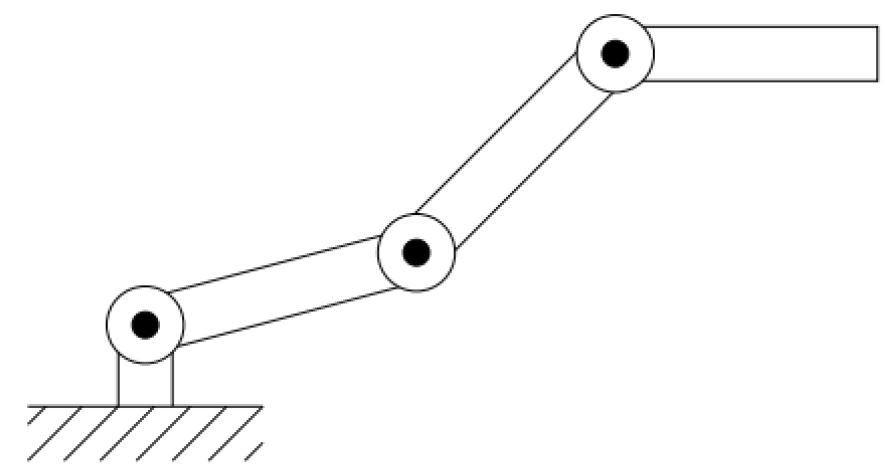
\includegraphics{1-Ejercicio_2_1_enunciado.JPG}}
    \end{adjustbox}
    \caption{Robot planar de 3 articulaciones rotacionales (Spong 2005).}
\end{figure}

\begin{figure}[H]
    \centering
    \begin{adjustbox}{scale = 0.5, max width=\columnwidth}
        \framebox{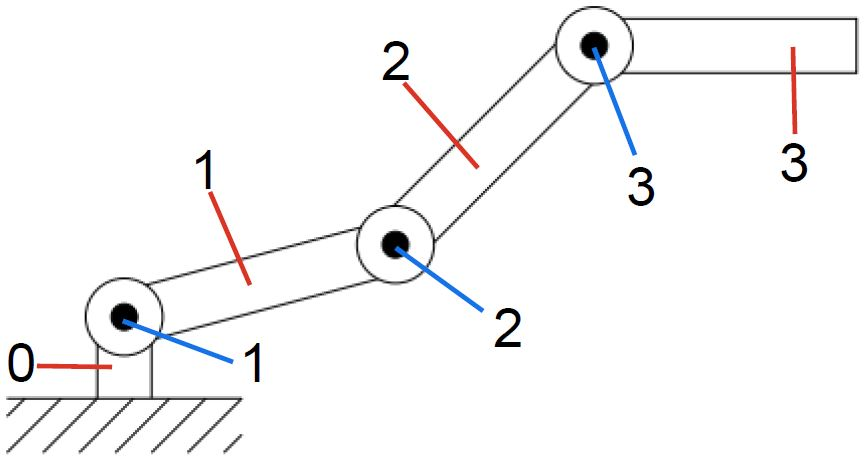
\includegraphics{2-Ejercicio_2_1_eslabones_articulaciones.JPG}}
    \end{adjustbox}
    \caption{Identificación de eslabones y articulaciones.}
\end{figure}

\begin{figure}[H]
    \centering
    \begin{adjustbox}{scale = 0.6, max width=\columnwidth}
        \framebox{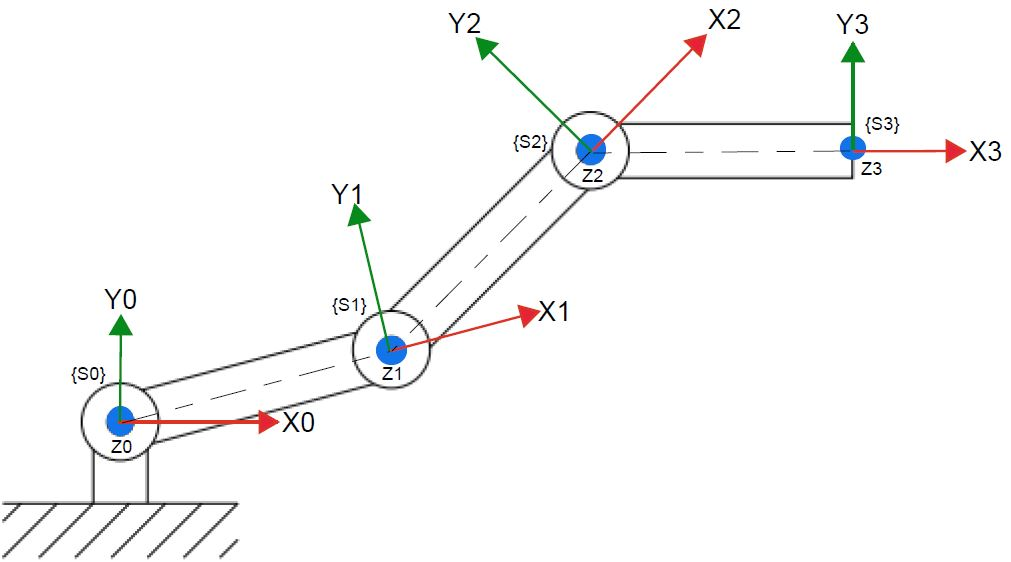
\includegraphics{3-Ejercicio_2_1_sistemas.JPG}}
    \end{adjustbox}
    \caption{Definición de los sistemas.}
\end{figure}

\begin{figure}[H]
    \centering
    \begin{adjustbox}{scale = 0.58, max width=\columnwidth}
        \framebox{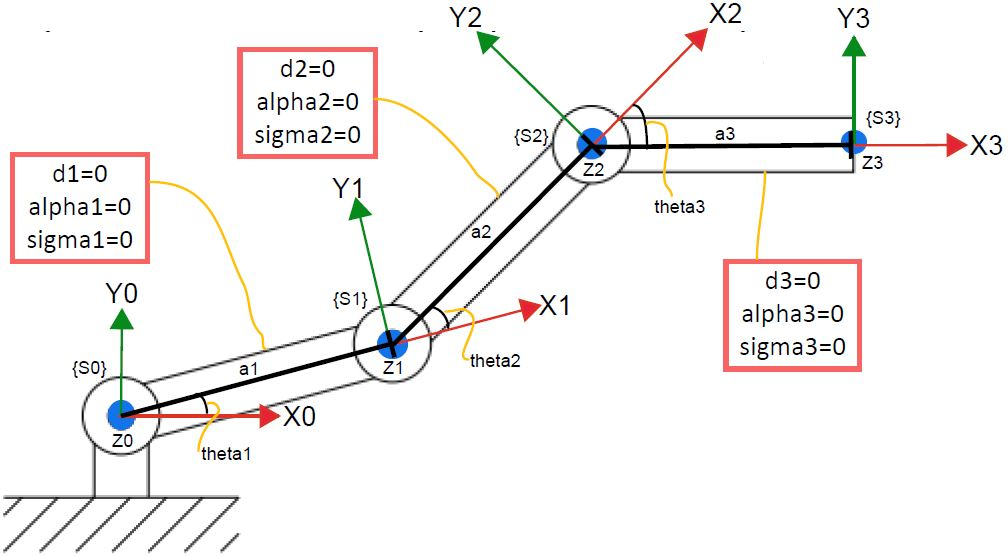
\includegraphics{4-Ejercicio_2_1_DH.JPG}}
    \end{adjustbox}
    \caption{Aplicación de la convención DH.}
\end{figure}

\begin{table}[H]
    \centering
    \begin{tabular}{|c|c|c|c|c|c|}
    \hline
    Sistema & $\theta$ & $d$ & $a$         & $\alpha$ & $\sigma$ \\ \hline
    1       & $q_1$     & 0   & $l_{esl1}$  & 0        & 0        \\ \hline
    2       & $q_2$     & 0   & $l_{esl2}$  & 0        & 0        \\ \hline
    3       & $q_3$     & 0   & $l_{esl3}$  & 0        & 0        \\ \hline
    \end{tabular}
    \caption{Síntesis de la convención DH.}
\end{table}

\subsection{Inciso 2}
\label{subsec: robot 2}

\begin{figure}[H]
    \centering
    \begin{adjustbox}{scale = 0.5, max width=\columnwidth}
        \framebox{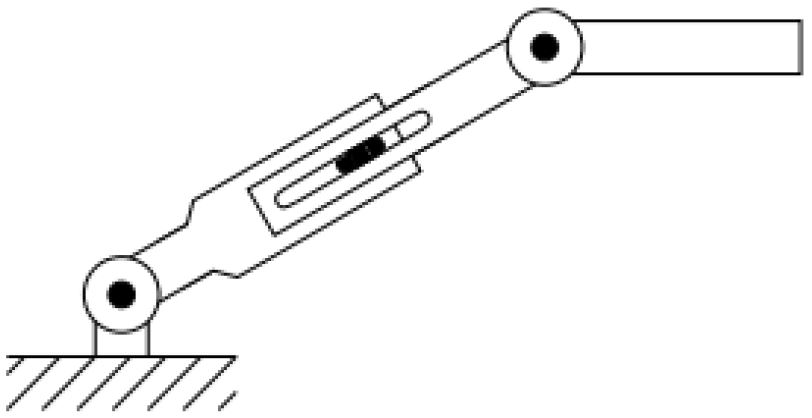
\includegraphics{5-Ejercicio_2_2_enunciado.JPG}}
    \end{adjustbox}
    \caption{Robot planar con 3 articulaciones: rotación, traslación, rotación (Spong 2005).}
\end{figure}

\begin{figure}[H]
    \centering
    \begin{adjustbox}{scale = 0.5, max width=\columnwidth}
        \framebox{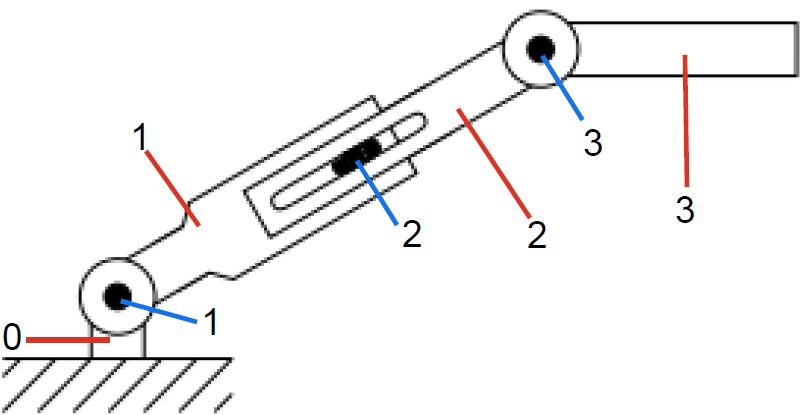
\includegraphics{6-Ejercicio_2_2_eslabones_articulaciones.JPG}}
    \end{adjustbox}
    \caption{Identificación de eslabones y articulaciones.}
\end{figure}

\begin{figure}[H]
    \centering
    \begin{adjustbox}{scale = 0.5, max width=\columnwidth}
        \framebox{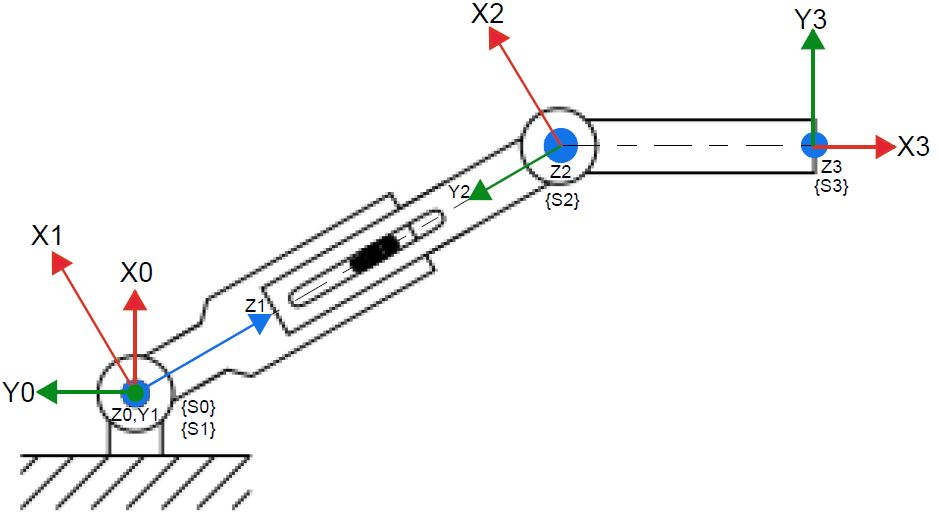
\includegraphics{7-Ejercicio_2_2_sistemas.JPG}}
    \end{adjustbox}
    \caption{Definición de los sistemas.}
\end{figure}

\begin{figure}[H]
    \centering
    \begin{adjustbox}{scale = 0.85, max width=\columnwidth}
        \framebox{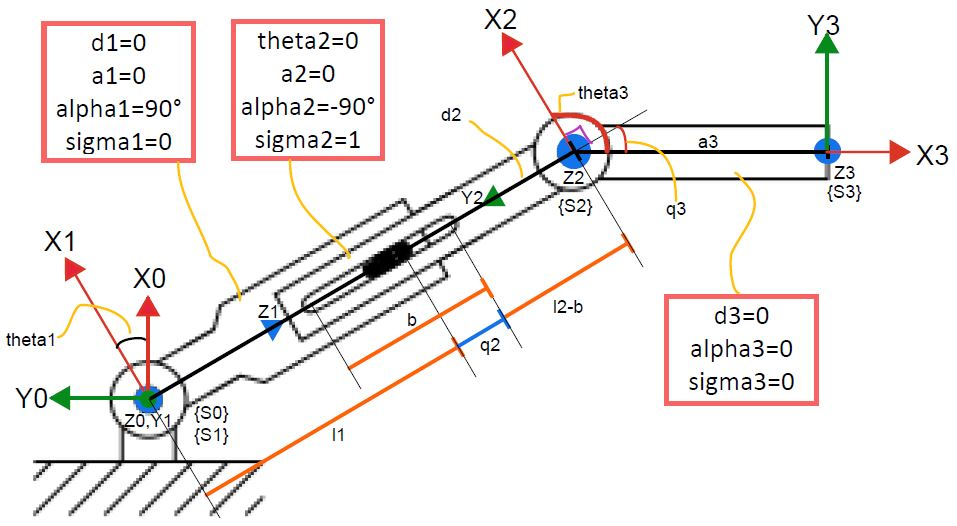
\includegraphics{8-Ejercicio_2_2_DH.JPG}}
    \end{adjustbox}
    \caption{Aplicación de la convención DH.}
    \label{robot 2 convencion}
\end{figure}

\begin{table}[H]
    \centering
    \begin{tabular}{|c|c|c|c|c|c|}
    \hline
    Sistema & $\theta$          & $d$                               & $a$         & $\alpha$     & $\sigma$ \\ \hline
    1       & $q_1$             & 0                                 & $0$         & $90^\circ$   & 0        \\ \hline
    2       & $0$               & $q_2 + l_{esl1} + l_{esl2} - b$   & $0$         & $-90^\circ$  & 1        \\ \hline
    3       & $q_3 - 90^\circ$  & 0                                 & $l_{esl3}$  & 0            & 0        \\ \hline
    \end{tabular}
    \caption{Síntesis de la convención DH.}
    \label{dh robot 2}
\end{table}

\subsection{Inciso 3}
\label{subsec: robot 3}

\begin{figure}[H]
    \centering
    \begin{adjustbox}{scale = 0.7, max width=\columnwidth}
        \framebox{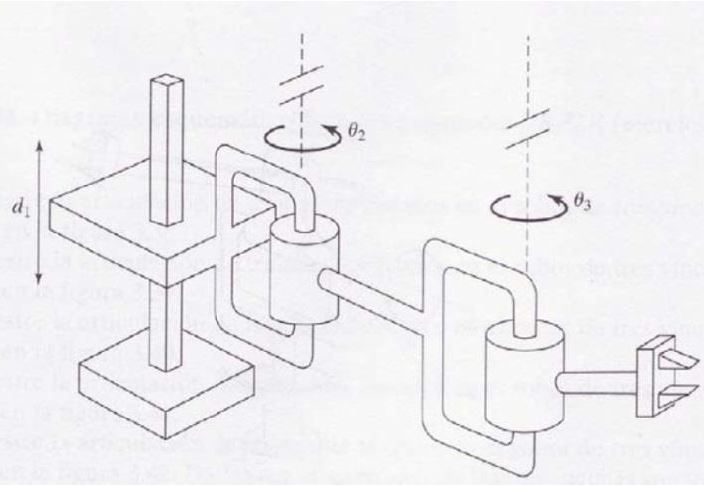
\includegraphics{9-Ejercicio_2_3_enunciado.JPG}}
    \end{adjustbox}
    \caption{Robot de 3 articulaciones: traslación, rotación, rotación (Craig 2006)}
\end{figure}

\begin{figure}[H]
    \centering
    \begin{adjustbox}{scale = 0.7, max width=\columnwidth}
        \framebox{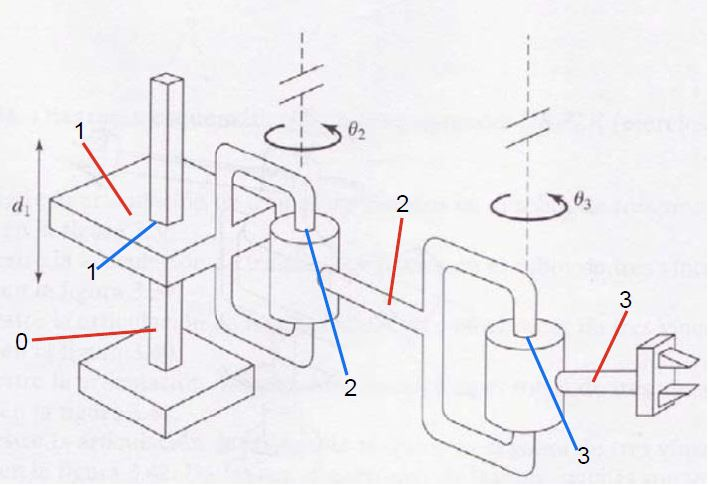
\includegraphics{10-Ejercicio_2_3_eslabones_articulaciones.JPG}}
    \end{adjustbox}
    \caption{Identificación de eslabones y articulaciones.}
\end{figure}

\begin{figure}[H]
    \centering
    \begin{adjustbox}{scale = 0.66, max width=\columnwidth}
        \framebox{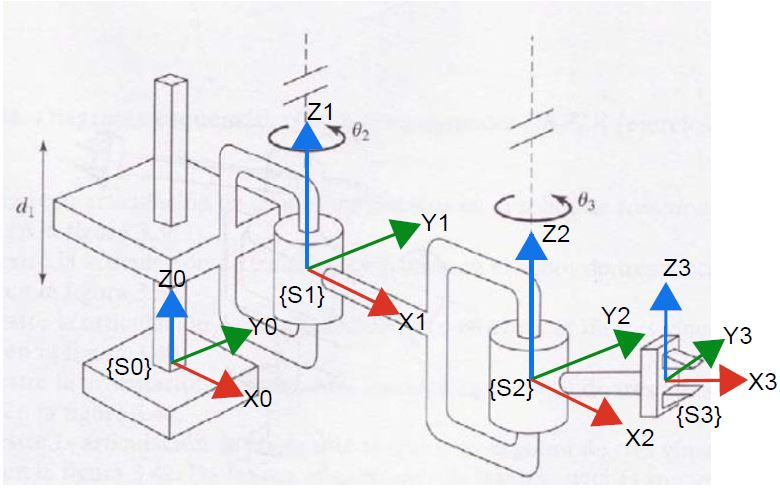
\includegraphics{11-Ejercicio_2_3_sistemas.JPG}}
    \end{adjustbox}
    \caption{Definición de los sistemas.}
\end{figure}

\begin{figure}[H]
    \centering
    \begin{adjustbox}{scale = 0.66, max width=\columnwidth}
        \framebox{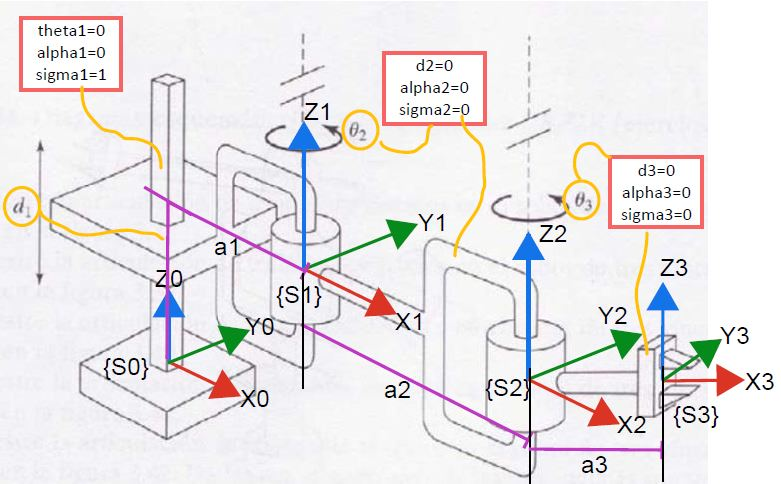
\includegraphics{12-Ejercicio_2_3_DH.JPG}}
    \end{adjustbox}
    \caption{Aplicación de la convención DH.}
\end{figure}

\begin{table}[H]
    \centering
    \begin{tabular}{|c|c|c|c|c|c|}
    \hline
    Sistema & $\theta$  & $d$ & $a$         & $\alpha$ & $\sigma$ \\ \hline
    1       & $0$       & $d_1$ & $l_{esl1}$  & 0      & 1        \\ \hline
    2       & $q_2$     & 0   & $l_{esl2}$  & 0        & 0        \\ \hline
    3       & $q_3$     & 0   & $l_{esl3}$  & 0        & 0        \\ \hline
    \end{tabular}
    \caption{Síntesis de la convención DH.}
\end{table}

\section{Ejercicio 3}
\textbf{Determine los parámetros DH de cada uno de los siguientes robots reales. Analice
cada uno de ellos y obtenga los datos necesarios de su geometría a partir de la información
gratuita que el fabricante pone a disposición en su página web. Si existe más de un modelo
para cada caso seleccione uno, cualquiera.}

\subsection{SCARA IRB 910SC-3/0.45 (ABB)}
\label{subsec: robot 4}

\begin{figure}[H]
    \centering
    \begin{adjustbox}{scale = 0.662, max width=\columnwidth}
        \framebox{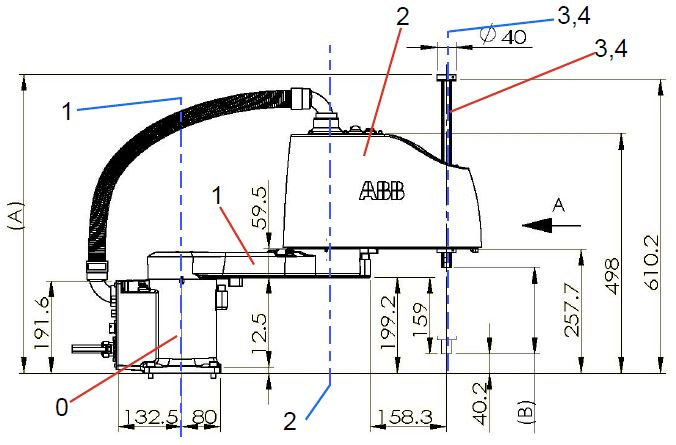
\includegraphics{13-Ejercicio_3_1_eslabones_articulaciones.JPG}}
    \end{adjustbox}
    \caption{Identificación de eslabones y articulaciones.}
    \label{scara_eslabones_articulaciones}
\end{figure}

\begin{figure}[H]
    \centering
    \begin{adjustbox}{scale = 0.662, max width=\columnwidth}
        \framebox{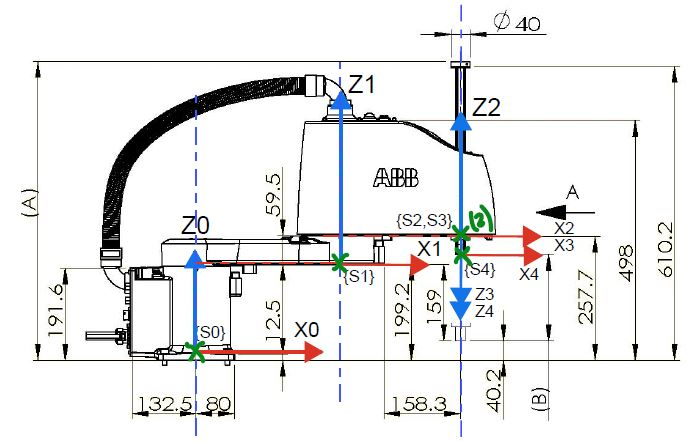
\includegraphics{14-Ejercicio_3_1_sistemas_lateral.JPG}}
    \end{adjustbox}
    \caption{Definición de sistemas vista lateral.}
    \label{scara_sistemas_lateral}
\end{figure}

Como se puede ver en las \cref{scara_eslabones_articulaciones}, \cref{scara_sistemas_lateral} y \cref{scara_sistemas_superior},
hemos separado al par cilíndrico en el extremo del robot por un par de rotación más un par prismático
y hemos considerado un sistema de referencia independiente para cada uno (\{S2\} y \{S3\}).

\begin{figure}[H]
    \centering
    \begin{adjustbox}{scale = 0.7, max width=\columnwidth}
        \framebox{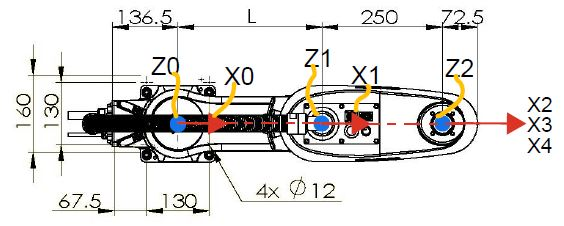
\includegraphics{15-Ejercicio_3_1_sistemas_superior.JPG}}
    \end{adjustbox}
    \caption{Definición de los sistemas vista superior.}
    \label{scara_sistemas_superior}
\end{figure}

Los parámetros para la convención DH se resaltaron en las \cref{DH_superior} y \cref{DH_lateral}
con cuadros de color violeta para las dimensiones en milímetros y con cuadros en rojo
para la denominación de los parámetros; mientras que aquellos parámetros que no se indican en las figuras
se colocan directamente en la \cref{sintesis_DH_scara}. En la \cref{DH_lateral} también se indica en forma
de árbol la cuenta para determinar $d_4$.

\begin{figure}[H]
    \centering
    \begin{adjustbox}{scale = 0.66, max width=\columnwidth}
        \framebox{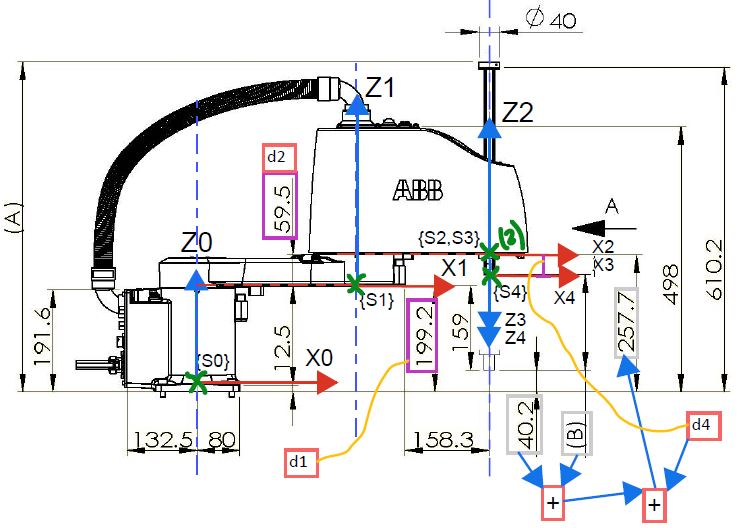
\includegraphics{16-Ejercicio_3_1_DH_lateral.JPG}}
    \end{adjustbox}
    \caption{Aplicación de la convención DH vista lateral.}
    \label{DH_lateral}
\end{figure}

El eje $X_3$ correspondiente al par prismático y el $X_4$ correspondiente al efector final, se mantienen alineados
con una línea de referencia inicial sobre la transversal al eslabón final del robot.

\begin{figure}[H]
    \centering
    \begin{adjustbox}{scale = 0.6, max width=\columnwidth}
        \framebox{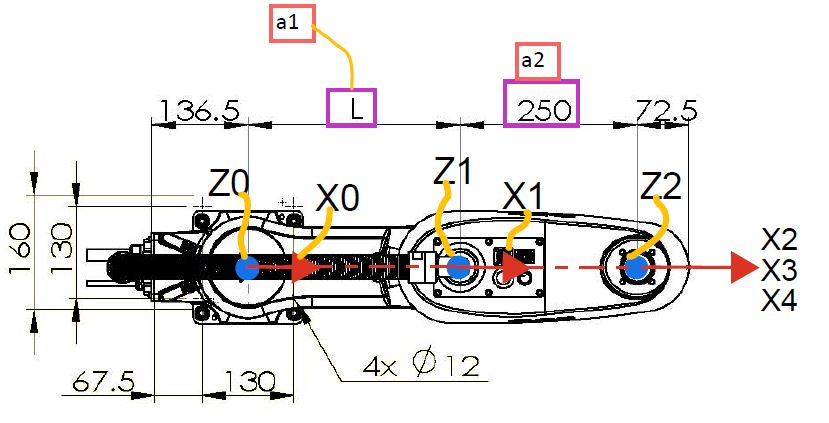
\includegraphics{17-Ejercicio_3_1_DH_superior.JPG}}
    \end{adjustbox}
    \caption{Aplicación de la convención DH vista superior.}
    \label{DH_superior}
\end{figure}

\begin{figure}[H]
    \centering
    \begin{adjustbox}{scale = 0.66, max width=\columnwidth}
        \framebox{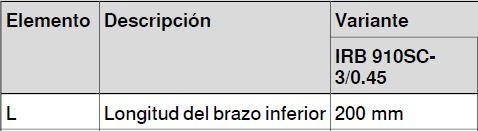
\includegraphics{18-Ejercicio_3_1_DH_parametros_dsh.JPG}}
    \end{adjustbox}
    \caption{parámetros 1.}
\end{figure}

\begin{figure}[H]
    \centering
    \begin{adjustbox}{scale = 0.66, max width=\columnwidth}
        \framebox{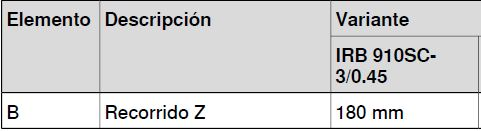
\includegraphics{19-Ejercicio_3_1_DH_parametros_dsh.JPG}}
    \end{adjustbox}
    \caption{parámetros 2.}
    \label{rango lineal scara}
\end{figure}

\begin{table}[H]
    \centering
    \begin{tabular}{|c|c|c|c|c|c|}
    \hline
    Sistema & $\theta$  & $d$           & $a$    & $\alpha$ & $\sigma$ \\ \hline
    1       & $q_1$     & $199.2$       & $200$  & 0        & 0        \\ \hline
    2       & $q_2$     & $59.5$        & $250$  & 0        & 0        \\ \hline
    3       & $q_3$     & $0$           & $0$    & 180°      & 0        \\ \hline
    4       & $0$       & $37.5 + q_4$  & $0$    & 0        & 1        \\ \hline
    \end{tabular}
    \caption{Síntesis de la convención DH.}
    \label{sintesis_DH_scara}
\end{table}

\subsection{Paint Mate 200iA (FANUC)}
\label{subsec: robot 5}

Aplicamos la convención DH directamente como se muestra en las \cref{DH FANUC overview} y \cref{DH FANUC lateral}..
En las que se ha identificado los sistemas de referencias para cada articulación y para el efector final
y se han resaltado los parámetros del robot que son útiles para la definición de la matriz de transformación 
homogénea según DH.

\begin{figure}[H]
    \centering
    \begin{adjustbox}{scale = 0.9, max width=\columnwidth}
        \framebox{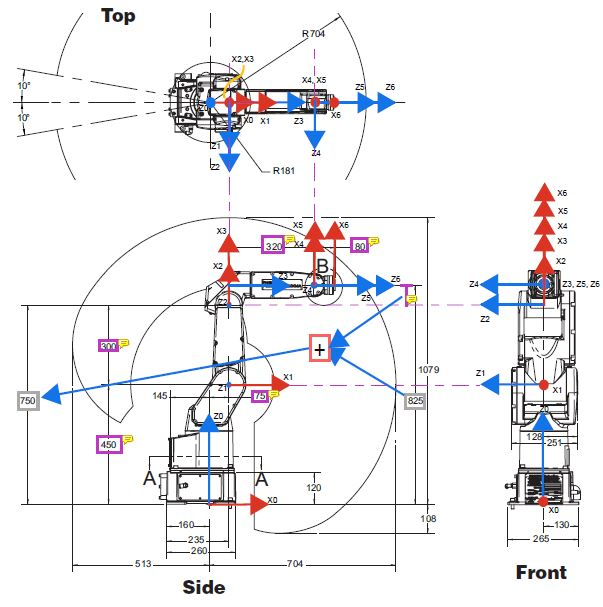
\includegraphics{20-Ejercicio_3_2_DH_parametros_dsh_overview.JPG}}
    \end{adjustbox}
    \caption{Aplicación de la convención DH overview.}
    \label{DH FANUC overview}
\end{figure}

\begin{figure}[H]
    \centering
    \begin{adjustbox}{scale = 0.65, max width=\columnwidth}
        \framebox{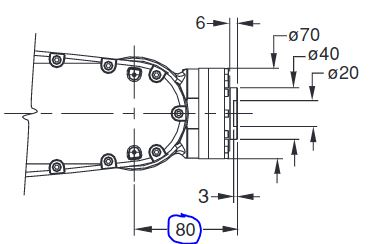
\includegraphics{22-Ejercicio_3_2_DH_parametros_dsh_wrist.JPG}}
    \end{adjustbox}
    \caption{Datos de la muñeca.}
    \label{DH FANUC muñeca}
\end{figure}

\begin{figure}[H]
    \centering
    \begin{adjustbox}{scale = 0.9, max width=\columnwidth}
        \framebox{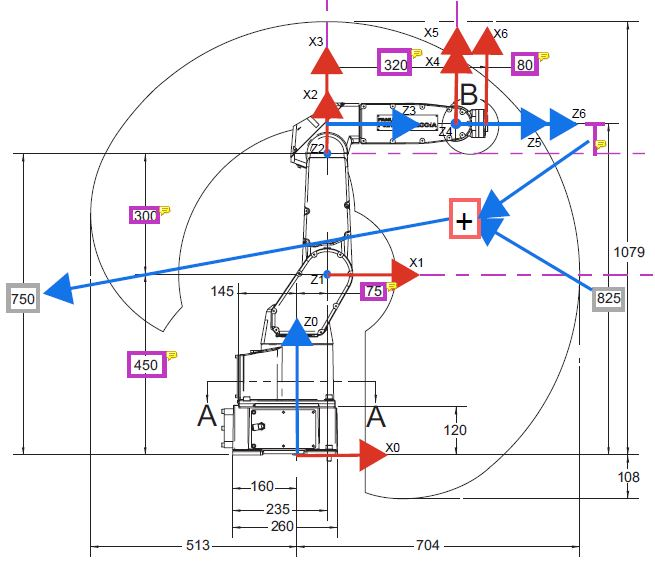
\includegraphics{21-Ejercicio_3_2_DH_parametros_dsh_side.JPG}}
    \end{adjustbox}
    \caption{Aplicación de la convención DH vista lateral.}
    \label{DH FANUC lateral}
\end{figure}

\begin{table}[H]
    \centering
    \begin{tabular}{|c|c|c|c|c|c|}
    \hline
    Sistema & $\theta$          & $d$    & $a$   & $\alpha$    & $\sigma$ \\ \hline
    1       & $q_1$             & $450$  & $75$  & $90^\circ$  & 0        \\ \hline
    2       & $90^\circ + q_2$  & $0$    & $300$ & $0$         & 0        \\ \hline
    3       & $q_3$             & $0$    & $75$  & $90^\circ$  & 0        \\ \hline
    4       & $q_4$             & $320$  & $0$   & $-90^\circ$ & 0        \\ \hline
    5       & $q_5$             & $0$    & $0$   & $90^\circ$  & 0        \\ \hline
    6       & $q_6$             & $80$   & $0$   & $0$         & 0        \\ \hline
    \end{tabular}
    \caption{Síntesis de la convención DH.}
    \label{sintesis DH FANUC}
\end{table}

\subsection{LBR iiwa 7 R800 (KUKA)}
\label{subsec: robot 6}

\begin{figure}[H]
    \centering
    \begin{adjustbox}{scale = 0.7, max width=\columnwidth}
        \framebox{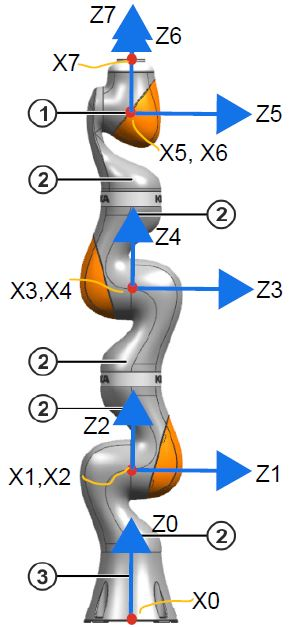
\includegraphics{23-Ejercicio_3_3_sistemas_lateral.JPG}}
    \end{adjustbox}
    \caption{Definición de sistemas vista lateral.}
    \label{KUKA sistemas lateral}
\end{figure}

\begin{figure}[H]
    \centering
    \begin{adjustbox}{scale = 0.9, max width=\columnwidth}
        \framebox{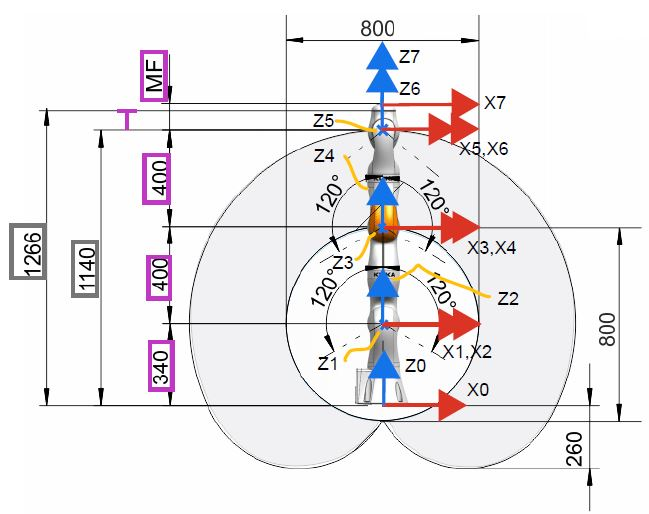
\includegraphics{24-Ejercicio_3_3_sistemas_frontal.JPG}}
    \end{adjustbox}
    \caption{Aplicación de la convención DH vista frontal.}
    \label{DH KUKA}
\end{figure}

\begin{table}[H]
    \centering
    \begin{tabular}{|c|c|c|c|c|c|}
    \hline
    Sistema & $\theta$          & $d$    & $a$   & $\alpha$    & $\sigma$ \\ \hline
    1       & $q_1$             & $340$  & $0$   & $90^\circ$  & 0        \\ \hline
    2       & $q_2$             & $0$    & $0$   & $-90^\circ$ & 0        \\ \hline
    3       & $q_3$             & $400$  & $0$   & $90^\circ$  & 0        \\ \hline
    4       & $q_4$             & $0$    & $0$   & $-90^\circ$ & 0        \\ \hline
    5       & $q_5$             & $400$  & $0$   & $90^\circ$  & 0        \\ \hline
    6       & $q_6$             & $0$    & $0$   & $-90^\circ$ & 0        \\ \hline
    7       & $q_7$             & $MF$   & $0$   & $0$         & 0        \\ \hline
    \end{tabular}
    \caption{Síntesis de la convención DH.}
    \label{sintesis DH KUKA}
\end{table}

\section{Ejercicio 4}
\textbf{Tome el robot 1 del punto anterior y escriba al menos 2 conjuntos de parámetros
DH diferentes que lo representen.}

Para conseguir otro juego de parámetros de DH nuevamente dividimos
el par cilíndrico en un par prismático y un par de rotación, pero ahora
tomamos el par prismático antes que el par de rotación en la cadena cinemática,
de esta manera, los parámetros DH son los que se muestran en \cref{parametros DH2}.

\begin{table}[H]
    \centering
    \begin{tabular}{|c|c|c|c|c|c|}
    \hline
    Sistema & $\theta$  & $d$           & $a$    & $\alpha$ & $\sigma$ \\ \hline
    1       & $q_1$     & $199.2$       & $200$  & 0        & 0        \\ \hline
    2       & $q_2$     & $59.5$        & $250$  & 0        & 0        \\ \hline
    3       & $0$       & $q_3$         & $0$    & 180°     & 1        \\ \hline
    4       & $q_4$     & $37.5$        & $0$    & 0        & 0        \\ \hline
    \end{tabular}
    \caption{Parámetros DH alternativos.}
    \label{parametros DH2}
\end{table}
En este caso, se toma el eje $X_3$, correspondiente el par de rotación,
en la misma dirección que el eje $X_2$ y el eje $X_4$, correspondiente al efector final,
en la dirección que una línea de referencia sobre la transversal al eslabón final del robot.

\section{Ejercicio 5.}
\textbf{Escriba un script de Matlab para cada robot del trabajo práctico. Use el toolbox de
Peter Corke para definirlos - clase (SerialLink) - y haga un plot de cada uno (SerialLink.plot).
Verifique gráficamente que sea el correcto mediante el movimiento de las articulaciones
(SerialLink.teach). Asigne medidas unitarias o genéricas si no dispone de 
reales}


\subsection{Robot en \cref{subsec: robot 1}}
\begin{itemize}
    \item Se toman longitudes unitarias de los eslabones.
    \item No se asignan offset de las variables articulares.
    \item Los límites articulares son de $\left(0^\circ; 180^\circ\right)$, $\left(-90^\circ; 270^\circ\right)$ y $\left(-90^\circ; 270^\circ\right)$ para las articulaciones 1, 2 y 3 respectivamente.
\end{itemize}

Verificación gráfica en \cref{teach robot 1}.

\begin{figure}[htpb]
    \centering
    \begin{adjustbox}{max width=\columnwidth}
        \framebox{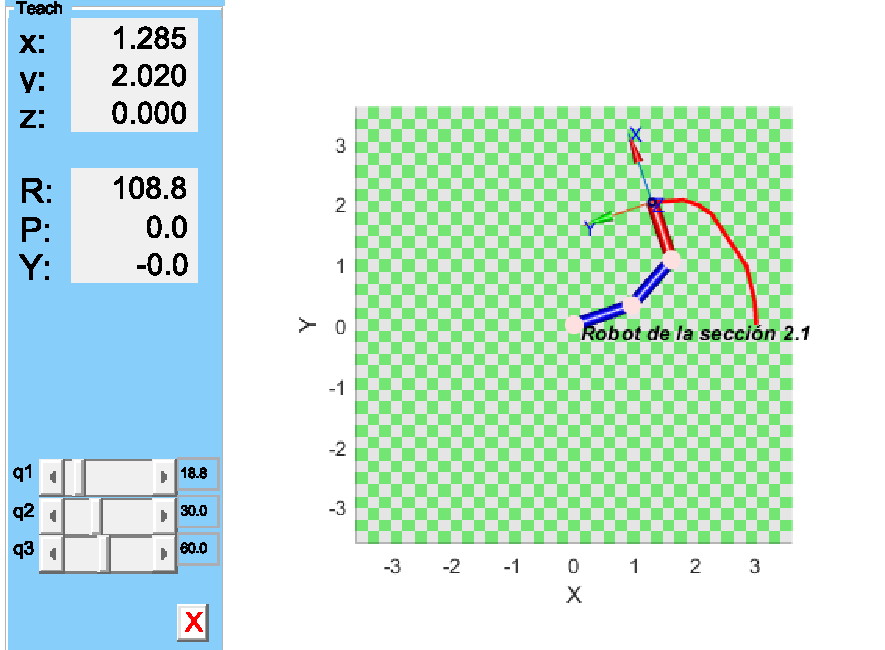
\includegraphics{25-Ejercicio_5_1.pdf}}
    \end{adjustbox}
    \caption{SerialLink.plot() y SerialLink.teach() robot 1}
    \label{teach robot 1}
\end{figure}

\subsection{Robot en \cref{subsec: robot 2}}
\begin{itemize}
    \item Se toman longitudes genericas de los eslabones.
    \item De la \cref{dh robot 2} se toman offsets de $0^\circ$, $0.5$ y $-90^\circ$ para las articulaciones 1, 2 y 3 respectivamente.
    \item Los límites articulares son de $\left(0^\circ; 180^\circ\right)$, $\left(0.5; 1\right)$ y $\left(-90^\circ; 270^\circ\right)$ para las articulaciones 1, 2 y 3 respectivamente.
    \item Como se puede observar en \cref{robot 2 convencion} hay una rotaión del sistema base de $90^\circ$ alrededor del eje z.
\end{itemize}

Verificación gráfica en \cref{teach robot 2}.

\begin{figure}[htpb]
    \centering
    \begin{adjustbox}{max width=\columnwidth}
        \framebox{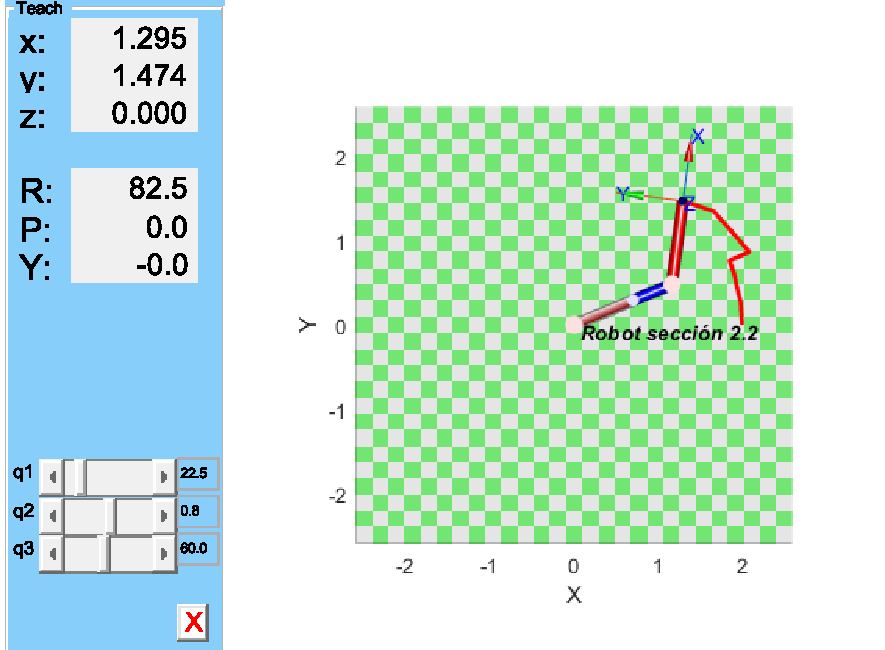
\includegraphics{26-Ejercicio_5_2.pdf}}
    \end{adjustbox}
    \caption{SerialLink.plot() y SerialLink.teach() robot 2}
    \label{teach robot 2}
\end{figure}

\subsection{Robot en \cref{subsec: robot 3}}
\begin{itemize}
    \item Se toman longitudes genericas de los eslabones.
    \item Se toma un offset de 1 en la primera articulación.
    \item Los límites articulares son de $\left(1; 2\right)$, $\left(-90^\circ; 270^\circ\right)$ y $\left(-90^\circ; 270^\circ\right)$ para las articulaciones 1, 2 y 3 respectivamente.
\end{itemize}

Verificación gráfica en \cref{teach robot 3}.

\begin{figure}[htpb]
    \centering
    \begin{adjustbox}{scale = 0.9, max width=\columnwidth}
        \framebox{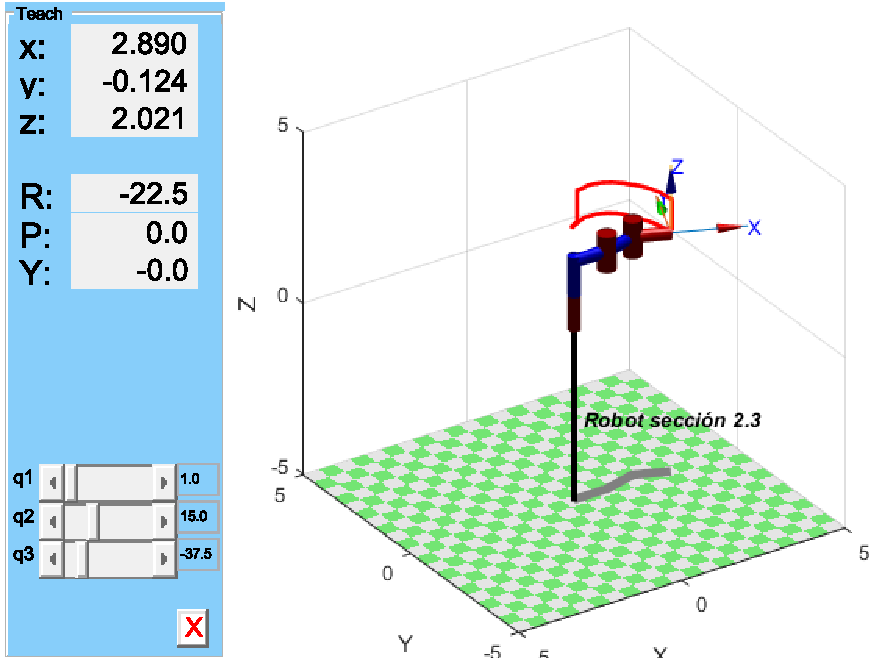
\includegraphics{27-Ejercicio_5_3.pdf}}
    \end{adjustbox}
    \caption{SerialLink.plot() y SerialLink.teach() robot 3}
    \label{teach robot 3}
\end{figure}

\subsection{Robot en \cref{subsec: robot 4}}
Todos los parámetros se obtienen de la \cref{sintesis_DH_scara}
y de las figuras en la \cref{subsec: robot 4}. Verificación gráfica en \cref{teach robot 4}.

Cuando se utilizan los parámetros alternativos que se dieron en la \cref{parametros DH2}
se obtiene lo que se indica en la \cref{teach robot 4 alt}.
En este caso, para el par prismático se toma un offset inicial igual a -180, que es el recorrido indicado en
\cref{rango lineal scara} y el rango de esa articulación se toma de 0 a 180 dado que no se pueden tener límites negativos en el rango de la variable articular prismática.

\begin{figure}[htpb]
    \centering
    \begin{adjustbox}{max width=\columnwidth}
        \framebox{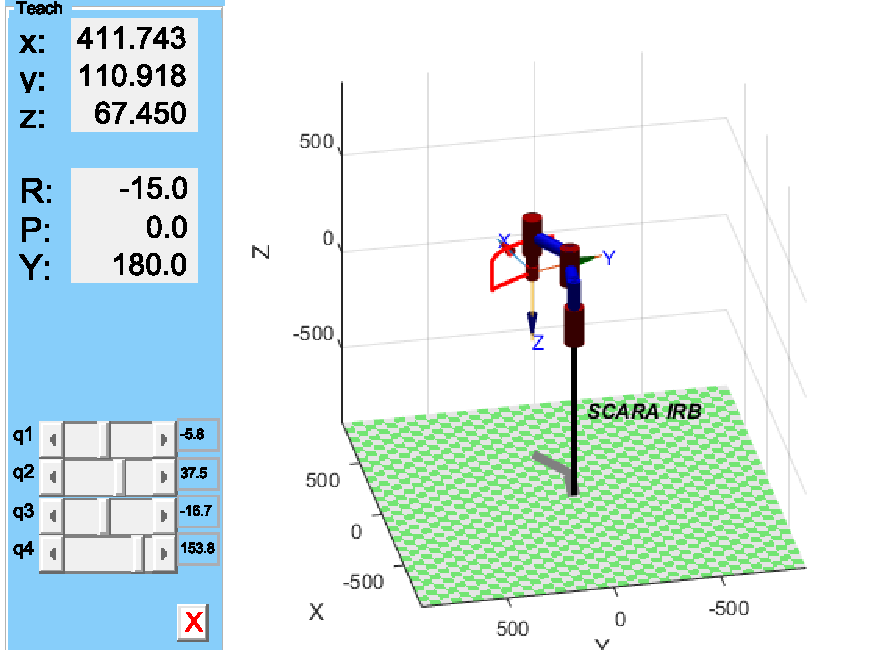
\includegraphics{28-Ejercicio_5_4.pdf}}
    \end{adjustbox}
    \caption{SerialLink.plot() y SerialLink.teach() robot 4}
    \label{teach robot 4}
\end{figure}

\begin{figure}[htpb]
    \centering
    \begin{adjustbox}{max width=\columnwidth}
        \framebox{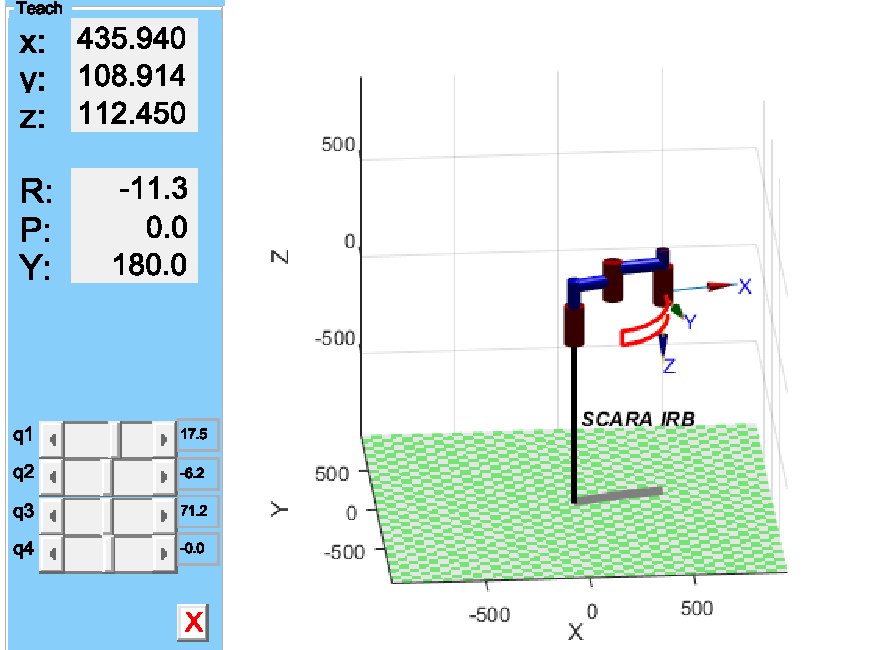
\includegraphics{29-Ejercicio_5_4_1.pdf}}
    \end{adjustbox}
    \caption{SerialLink.plot() y SerialLink.teach() robot 4 DH alternativo}
    \label{teach robot 4 alt}
\end{figure}

\subsection{Robot en \cref{subsec: robot 5}}
Verificación gráfica en la \cref{teach robot 5}.

\begin{figure}[htpb]
    \centering
    \begin{adjustbox}{max width=\columnwidth}
        \framebox{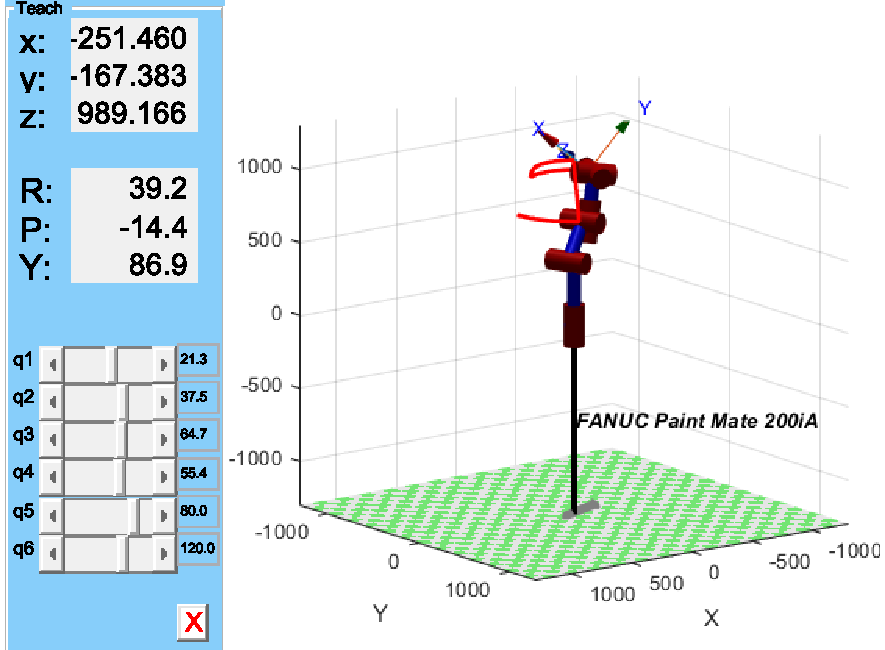
\includegraphics{30-Ejercicio_5_5.pdf}}
    \end{adjustbox}
    \caption{SerialLink.plot() y SerialLink.teach() robot 5}
    \label{teach robot 5}
\end{figure}
\end{document}

%\begin{equation*}
%    \prescript{O}{}{Rot_M} = 
%    \begin{bmatrix}
%        0.500 & -0.866\\
%        0.866 & 0.500
%    \end{bmatrix}
%\end{equation*}

%\begin{figure}[H]
%    \centering
%    \begin{adjustbox}{scale = 0.85, max width=\columnwidth}
%        \framebox{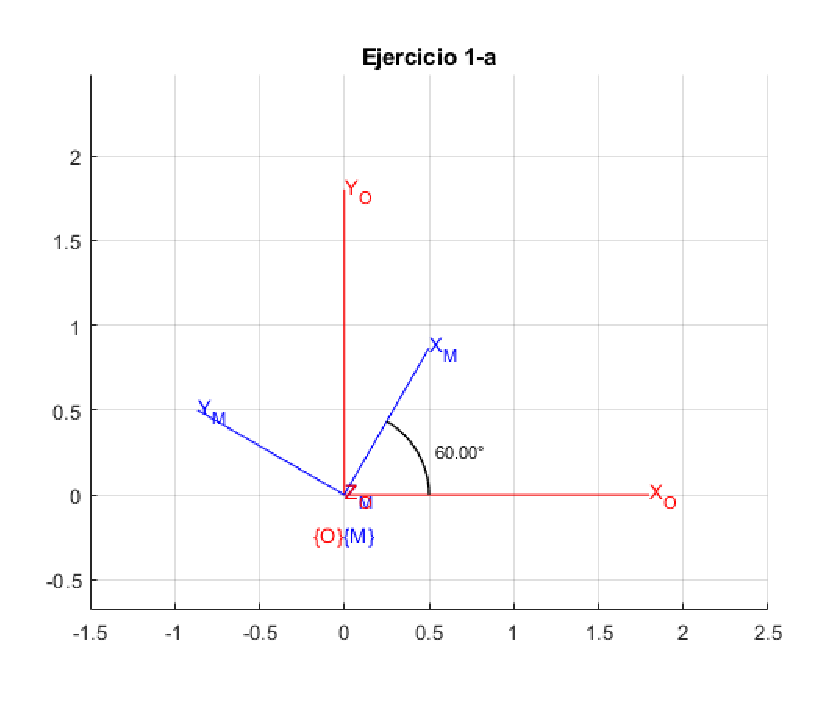
\includegraphics{1-Ejercicio_1_a.pdf}}
%    \end{adjustbox}
%    \caption{Sistema O y Sistema M superpuestos con indicación de ángulo de rotación.}
%\end{figure}

\end{document}